\chapter{Supplemental Material for Chapter \ref{chap:chapter 2}}

Additional supplemental material can be found in the published location at \url{https://doi.org/10.2337/db24-0497}. 

\begin{table}[ht]
    \centering
    \caption[Human variants in \texorpdfstring{\(PPARG\)}{PPARG} upstream of M135.]{\textbf{Human variants in \texorpdfstring{\(PPARG\)}{PPARG} upstream of M135.} Each variant encodes a frameshift (fs) that results in a termination (Ter) or a stop codon (*), and the protein consequence is relative to ENSP00000287820.6. The first variant, p.Thr41ProfsTer12, encodes a stop codon at amino acid 52 on Exon 1. The second variant, p.Ile45SerfsTer8, encodes a stop codon at amino acid 52. The third variant, p.Lys63GlnfsTer7, encodes a stop codon at amino acid 69. The fourth variant, p.Ser74TyrfsTer24, results in a stop codon at amino acid 97. The fifth variant, p.Tyr78Ter, encodes a stop codon at amino acid 78. The sixth variant, p.Phe65SerfsTer33, encodes a stop codon at amino acid 97. The seventh variant, p.Gln121*, encodes a stop codon at amino acid 121. All of these occur upstream of p.M135.
  }
    \begin{tabular}{|c|c|m{4.2cm}|m{2cm}|}
    \hline
        Variant ID (hg38) & Protein Consequence & Database & Sample Size \newline (n) \\ \hline
        3-12379738-GC-G & p.Thr41ProfsTer12 & All of Us & 245400 \\ \hline
        3-12379750-TG-T & p.Ile45SerfsTer8 & Regeneron Genetics Center (RGC) Million Exome & 983578 \\ \hline
        3-12379805-A-AT & p.Lys63GlnfsTer7 & 1000G & 2548 \\ \hline
        3-12379837-C-CATTT & p.Ser74TyrfsTer24 & All of Us & 245400 \\ \hline
        3-12379855-C-G & p.Tyr78Ter & RGC Million Exome & 983578 \\ \hline
        3-12379813-CT-C & p.Phe65SerfsTer33 & RGC Million Exome & 983578 \\ \hline
        3-12381372-C-T & p.Gln121* & Framingham Heart Study (FHS) & 1637 \\ \hline
    \end{tabular}
\end{table}


\begin{figure}[ht]
    \centering
    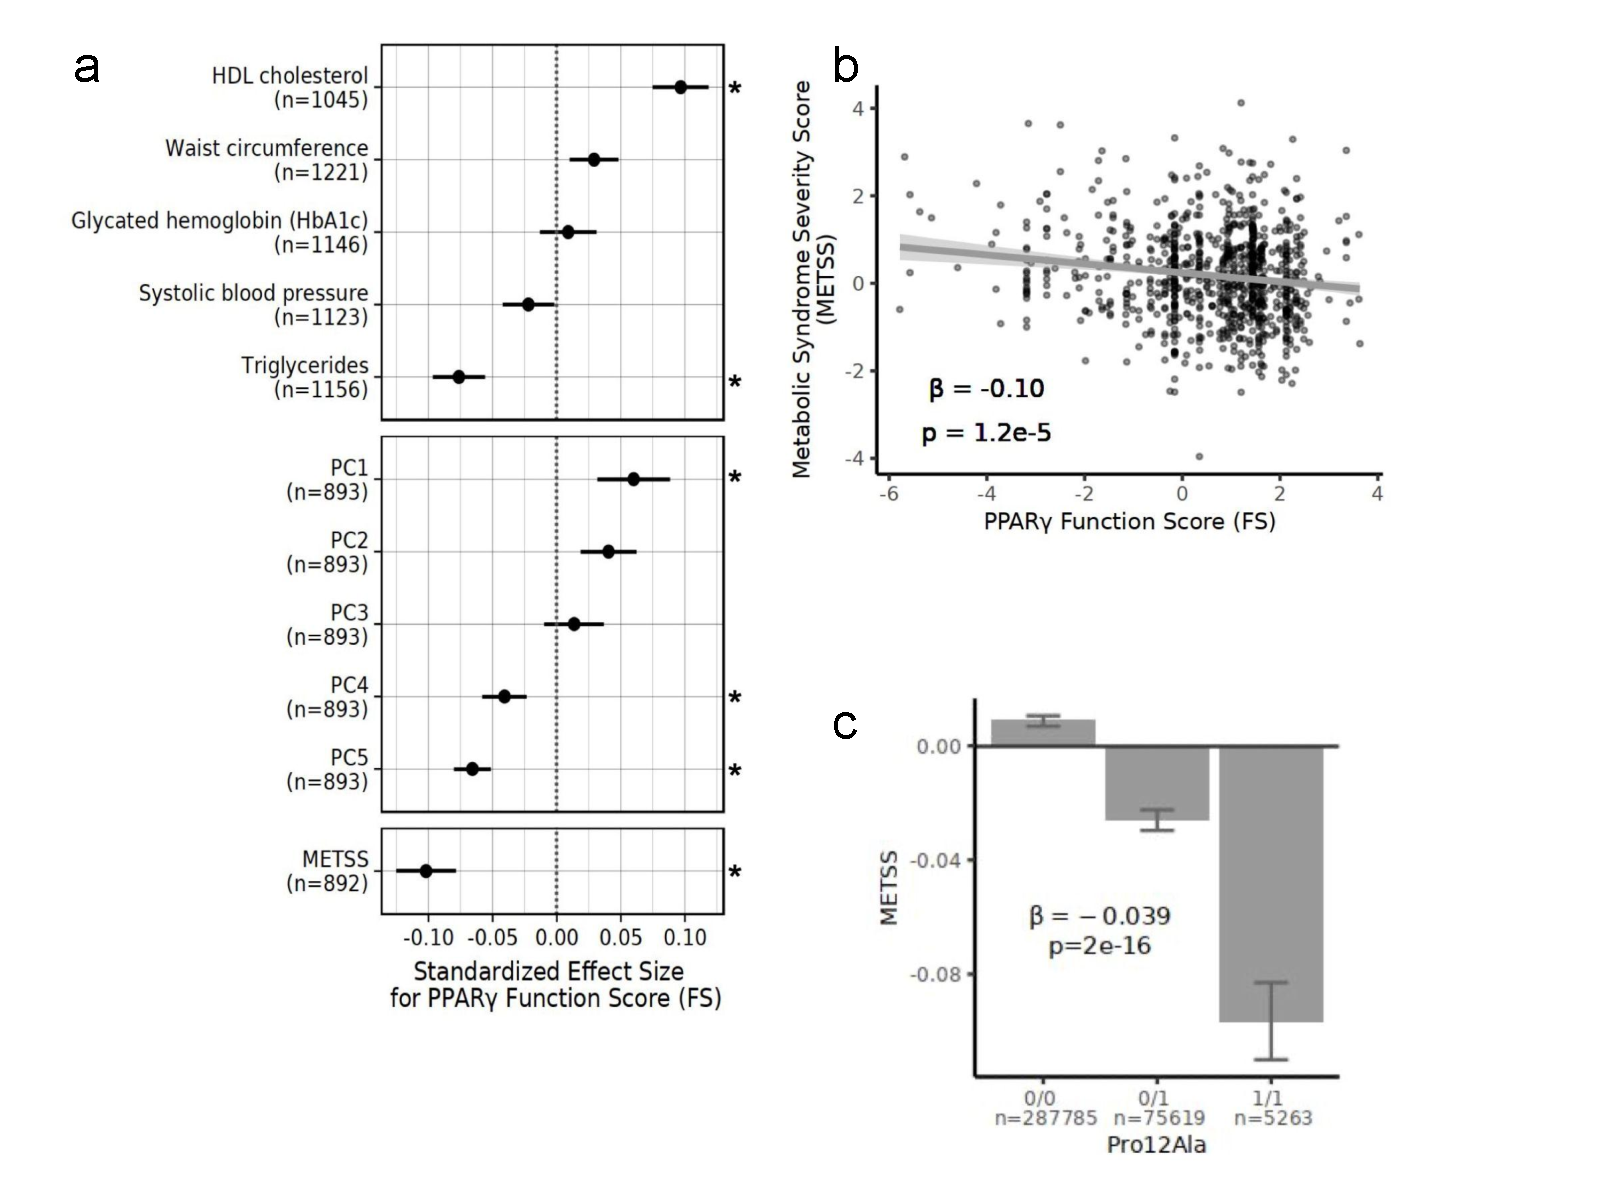
\includegraphics[width=\textwidth]{2_figures-and-files/FigS1.pdf}
    \caption[Aggregation of clinical phenotypes into a metabolic syndrome severity score (METSS).]{\textbf{Aggregation of clinical phenotypes into a metabolic syndrome severity score (METSS).} a. A metabolic syndrome severity score (METSS) was computed from five clinical phenotypes: serum HDL cholesterol, waist circumference, serum triglycerides, systolic blood pressure, and glycated hemoglobin (HbA1c). Regression coefficients for each phenotype against PPAR$\gamma$ function score (FS) are plotted with covariate adjustments for age, age2, sex, and 10 genetic principal components. Only serum triglycerides and HDL cholesterol show significant regression slopes. Analogous regression analysis was performed and plotted for principal components (PCs) derived from dimensionality reduction (i.e. PCA) performed on the five clinical phenotypes. PC1, PC4 and PC5 had significant effect sizes when regressed against the PPAR$\gamma$ FS. Standardized effect size (dot) and standard error (lines) are shown for each value; the sample size is the number of individuals with each phenotype/PC and the PPAR$\gamma$ FS, and significance was determined by p $<$ 0.05. Only 892 individuals were carriers of rare, protein-coding \(PPARG\) variants with PPAR$\gamma$ FS and had computable METSS. b. In carriers of \(PPARG\) missense variants with METSS (n=892), the metabolic syndrome severity score decreases with increasing PPAR$\gamma$ function (linear regression, effect size = -0.10, p=1.2e-5). c. Mean and sem of METSS by Pro12Ala genotype. METSS decreases with increasing alleles of the alternate, as modeled by METSS ~ number of alternate alleles, which has effect size of -0.039 and p-value=2e-16.
    }
\end{figure}
